\documentclass[varwidth=40cm]{standalone}
\usepackage{tikz}
\usetikzlibrary{patterns,decorations.pathreplacing}
\usepackage{style}

\begin{document}
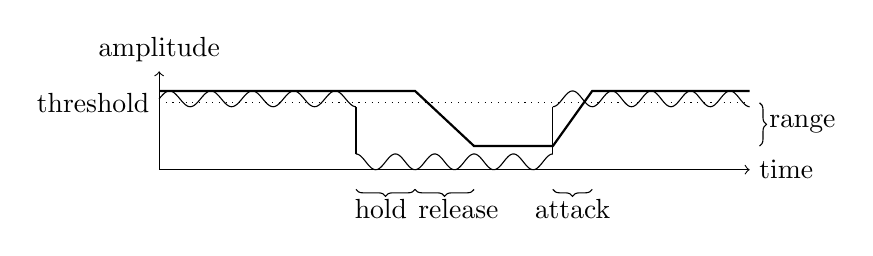
\begin{tikzpicture}[xscale=.5,yscale=1.]
  \draw[->] (0,0) -- (15,0) node[right] {time};
  \draw[->] (0,0) -- (0,1.25) node[above] {amplitude};
  \draw[dotted] (0,.85) node[left] {threshold} -- (15,.85);
  \draw[domain=0:5,samples=400] plot ({\x},{sin(\x*360*4.75/5)/10+.9});
  \draw[domain=5:10,samples=400] plot ({\x},{sin((\x+.25)*360)/10+.1});
  \draw[domain=10:15,samples=400] plot ({\x},{sin((\x-.25)*360)/10+.9});
  \draw (5,.8) -- (5,.2);
  \draw (10,.8) -- (10,.2);
  \draw[thick] (0,1) -- (6.5,1) -- (8,.3) -- (10,.3) -- (11,1) -- (15,1);
  \draw[decoration={brace,mirror}, decorate] (5,-.25) -- (6.5,-.25) node [pos=0.5,below] {hold~~};
  \draw[decoration={brace,mirror}, decorate] (6.5,-.25) -- (8,-.25) node [pos=0.5,below] {~~~release};
  \draw[decoration={brace,mirror}, decorate] (10,-.25) -- (11,-.25) node [pos=0.5,below] {attack};
  \draw[decoration={brace,mirror}, decorate] (15.25,.3) -- (15.25,.85) node [pos=0.5,right] {range};
\end{tikzpicture}
\end{document}
